\documentclass[main.tex]{subfiles} % Subfile-Class

%==============================================================================%
%                                   Subfile                                    %
%==============================================================================%

\begin{document}

\subsection{Sprintziele und Grobplanung}

Das Projekt ist in insgesamt 5 Sprints unterteilt. Diese umfassen eine
Vorbereitungsphase, 3 Arbeitsphasen und eine Abschlussphase.
Abbildung~\ref{fig:Grobplanung} zeigt die Grobplanung des Projekts auf Basis
eines Miro-Boards. Darin sind die einzelnen Sprints und deren Ziele grob
skizziert.

\begin{figure}[h]
    \centering
    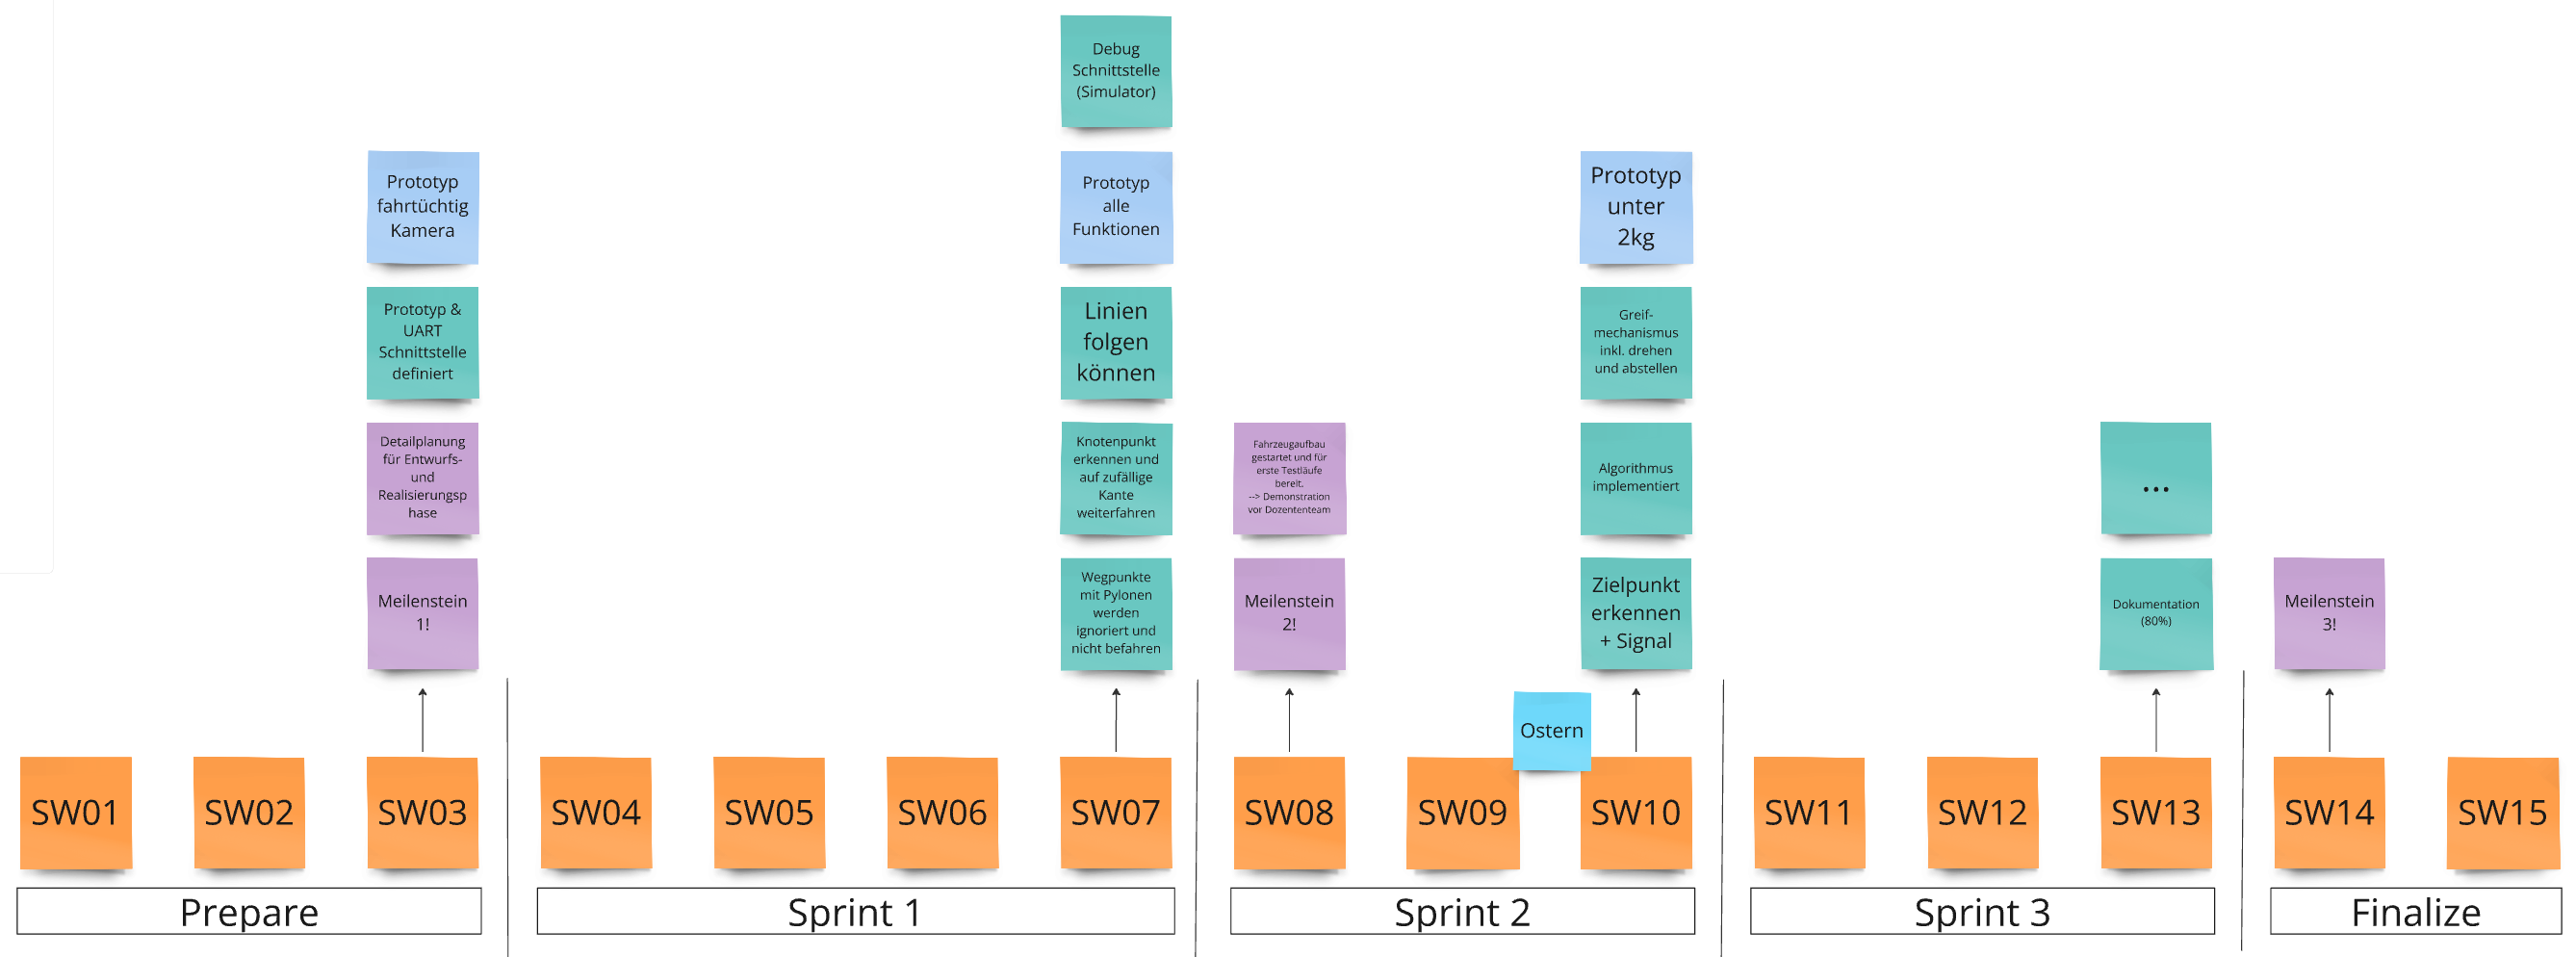
\includegraphics[width=1\textwidth]{./Grobplanung_MiroBoard.png}
    \caption{Grobplanung auf einem Miro-Board}~\label{fig:Grobplanung}
\end{figure}

Nachfolgend werden die einzelnen Sprintziele nochmals formuliert.

\subsubsection*{Sprintziel \textit{Prepare}}
Ziel der Vorprojektphase ist die Planung und Vorbereitung des Projektes sowie
der Bau eines ersten funktionsfähigen Prototyps.

Dieser erste Prototyp wird noch über keinerlei Funktionalität verfügen, mit
Ausnahme derer, die notwendig sind, um einer Linie zu folgen. Dementsprechend
wird die Grundplatte des Chassis gefertigt, sowie der
\textit{MotionController}, der \textit{RaspberryHAT} und das
\textit{PowerBoard} aufgebaut und grundlegend in Betrieb genommen.

Seitens der Informatik wird das Kommunikationsprotokoll zwischen den einzelnen
den einzelnen PCB's definiert und der Raspberry Pi mit der Kamera aufgesetzt
und in Betrieb genommen.

\subsubsection*{Sprintziel \textit{Sprint 1}}
Am Ende von Sprint 1, d.h. in Semesterwoche 7, muss das Fahrzeug in der Lage sein,
einer Linie zu folgen. Außerdem soll die Fahrzeugsteuerung in der Lage sein,
Knotenpunkte zu erkennen und auf einer zufälligen Kante weiterzufahren. Wegpunkte
mit Pylonen sollen ignoriert und nicht befahren werden.

Dazu muss die grundlegende Kommunikation zwischen dem MotionController und dem
RaspberryHAT funktionieren. Die Antriebssteuerung muss implementiert und
getestet werden.

In diesem Sprint wird die Greifeinheit sowohl mechanisch als auch elektronisch
aufgebaut. Der GripController ist also zusammengebaut und mit dem Greifer
verbunden. Eine funktionierende Greifeinheit ist jedoch noch nicht das Ziel
dieses Sprints.

\subsubsection*{Sprintziel \textit{Sprint 2}}
Der Schwerpunkt von Sprint 2 liegt auf der Inbetriebnahme der Greifeinheit sowie
auf der Ausarbeitung des Algorithmus zur Wegfindung.

Am Ende des Sprints soll das Fahrzeug in der Lage sein, Hindernisse zu greifen
und wieder abzusetzen sowie Zielpunkte zu erkennen und das Erreichen dieser zu
signalisieren.

Aus mechanischer Sicht soll das Fahrzeuggewicht am Ende des Sprints in
Semesterwoche 10 unter 2 kg liegen.

\subsection*{Sprintziel \textit{Sprint 3}}
Sprint 3 konzentriert sich auf die Projektdokumentation. Am Ende dieses Sprints,
in KW 13, ist die Meilensteinübergabe des 80\% Dokumentationsmeilensteins. Darüber
hinaus dient er als Puffer für kleinere Verbesserungen und Optimierungen sowie
Rückstände aus den vorangegangenen Sprints.

\subsection*{Sprintziel \textit{Finalize}}
In der Abschlussphase des Projekts, in den Semesterwochen 13 und 14, werden
abschließende Tests durchgeführt und die Dokumentation fertiggestellt. Am Ende
dieses Sprints muss das Fahrzeug Einsatzbereit für den Wettkampf sein.

\subsection{Detailplanung}
Wie im letzten Jahr wird die Detailplanung unseres Projekts mit dem Tool
\textit{GitHub-Projects} durchgeführt. Die Detailplanung kann unter folgendem
Link eingesehen werden:
\href{https://github.com/users/JulesBischof/projects/6/views/4}{GitHub-Project}.
Jede Disziplin teilt dabei die zu erreichenden Sprintziele in kleinere
Arbeitspakete auf. Sollte entgegen der Erwartung eine fehlende Berechtigung
festgestellt werden, so kann sich sich bei \textit{Julian Bischof} unter der
E-Mail-Adresse \textit{julian.bischof@stud.hslu.ch} gemeldet werden.

\end{document}
